%!TEX program = xelatex

\documentclass[compress]{beamer}
%--------------------------------------------------------------------------
% Common packages
%--------------------------------------------------------------------------

\definecolor{links}{HTML}{663000}
\hypersetup{colorlinks,linkcolor=,urlcolor=links}

\usepackage[english]{babel}
\usepackage{pgfpages} % required for notes on second screen
\usepackage{graphicx}

\usepackage{multicol}

\usepackage{tabularx,ragged2e}
\usepackage{booktabs}

\setlength{\emergencystretch}{3em}  % prevent overfull lines
\providecommand{\tightlist}{%
  \setlength{\itemsep}{0pt}\setlength{\parskip}{0pt}}


\usetheme{hri}

% Display the navigation bullet even without subsections
\usepackage{remreset}% tiny package containing just the \@removefromreset command
\makeatletter
\@removefromreset{subsection}{section}
\makeatother
\setcounter{subsection}{1}

\makeatletter
\let\beamer@writeslidentry@miniframeson=\beamer@writeslidentry
\def\beamer@writeslidentry@miniframesoff{%
  \expandafter\beamer@ifempty\expandafter{\beamer@framestartpage}{}% does not happen normally
  {%else
    % removed \addtocontents commands
    \clearpage\beamer@notesactions%
  }
}
\newcommand*{\miniframeson}{\let\beamer@writeslidentry=\beamer@writeslidentry@miniframeson}
\newcommand*{\miniframesoff}{\let\beamer@writeslidentry=\beamer@writeslidentry@miniframesoff}
\makeatother



\newcommand{\source}[2]{{\tiny\it Source: \href{#1}{#2}}}

\usepackage[normalem]{ulem}

\usepackage{tikz}
\usetikzlibrary{intersections,arrows,shapes,calc,mindmap,backgrounds,positioning,svg.path}

\tikzset{box/.style={
            draw, 
            fill=blue!20,
            fill opacity=0.8,
            thick,
            inner sep=0pt,
            minimum size=1cm,
            transform shape
        },
        finalbox/.style={
            draw, 
            fill=orange,
            fill opacity=0.8,
            thick,
            inner sep=0pt,
            minimum size=1cm,
            transform shape
        },
        dot/.style={
            draw,
            circle,
            fill=red!20,
            inner sep=0pt,
            minimum size=1cm,
            transform shape
        },
        axis/.style={
            thick,
            gray,
            font=\small},
        every to/.style={
            >=latex,
            dashed,
            thick
        }
    }


\graphicspath{{figs/}}

\title{ROS}
\subtitle{The Robot Operating System}

\date{}
\author{Séverin Lemaignan}
\institute{Bristol Robotics Lab\\{\bf University of West of England}}

\begin{document}

\licenseframe{github.com/severin-lemaignan/ros-presentation}

\maketitle

\miniframesoff

\miniframeson

\section[Intro]{ROS is not an operating system}

\begin{frame}{Instead, ROS is...}
    \begin{itemize}
        \item<1-> A fairly simple peer-to-peer message passing system designed with robotics in
            mind
        \item<2-> An API to this system (in several languages -- C++ and Python are
            1st tier)
        \item<3-> A set of standard message types that facilitate interoperability between modules
        \item<4> \bf{A middleware?}
        \item<5-> A set of conventions to write and package robotic softwares
        \item<6-> Deep integration of a few key open-source libraries (OpenCV, PCL, tf)
        \item<7-> A set of tools to run and monitor the nodes
        \item<8-> Engagement of a large academic community, leading to a library of thousands of nodes
    \end{itemize}
\end{frame}

\begin{frame}{ROS Ecosystem}
    \centering
    \resizebox{0.9\textwidth}{!}{%
        \vspace*{4cm}
        \begin{tikzpicture}

            \path[small mindmap,
                  level 1 concept/.append style={sibling angle=360/5}, 
                  level 2 concept/.append style={sibling angle=60}, 
                  concept color=hriWarmGreyLight,text=hriWarmGreyDark]

            node[concept] {\bf ROS}
            [clockwise from=-180]
            child[concept color=hriSec1Dark,text=white] { node[concept]{Middleware} 
                [clockwise from=-120]
                child[concept color=hriSec1CompDark,text=white] { node[concept]{Standard Interfaces} }
                child[concept color=hriSec3CompDark,text=white] { node[concept]{Nodes Management} }
                child[concept color=hriSec2Dark,text=white] { node[concept]{IPC} }
            }
            child[concept color=hriSec3Comp,text=white] { node[concept] {Standards and Conventions} }
            child[concept color=hriSec2CompDark,text=white] { node[concept]{Community}
                [clockwise from=90]
                child[concept color=hriSec2Comp,text=white] { node[concept]{Software engineering infrastructure} }
                child[concept color=hriSec1,text=white] { node[concept] {REPs} }
                child[concept color=hriSec3,text=white] { node[concept] {ROSCon} }
            }
            child[concept color=hriSec3Dark,text=white] { node[concept] {Large software library} 
                [clockwise from=0]
                child[concept color=hriSec2Dark,text=white] { node[concept] {Satellite libraries} }
            }
            child[concept color=hriSec3CompDark,text=white] { node[concept] {Tooling} };
        \end{tikzpicture}
    }
\end{frame}

\begin{frame}{}
    [we will revisit these slides at the end of the lecture]
\end{frame}

\section[Example]{A first example}

\begin{frame}{A simple image processing pipeline}

\begin{center}
\begin{tikzpicture}[
                    >=latex,
                    every edge/.style={->, draw, very thick},
                    service/.style={->, draw, very thick,dashed},
                    rosnode/.style={draw, font=\sf, node distance=0.5, rounded
                    corners, align=center, inner sep=5pt,fill=hriSec2Dark!50},
                    topic/.style={font=\tt, node distance=0.5, align=center, inner sep=5pt},
                    pic/.style={fill=none,draw=none}
                ]

    \node [rosnode] at (-4,0) (node1) {image acquisition};
    \node [rosnode] at (0,-2) (node2) {image processor};
    \node [rosnode] at (4,-4) (node3) {next processing};

        \node [topic] at (-4,-1.5) (topic3) {/image};
        \node [topic] at (-1,-3.5) (topic1) {/processed\_image};
        \path (node1) edge[bend right] (node2);
        \path (node2) edge[bend right] (node3);


    \uncover<2-> {

        \node at (-0,0) (a) {this is a \textbf{node}};
        \path[dashed] (a) edge (node1);
        \node at (-4.5,-3) (b) {this is a \textbf{topic}};
        \path[dashed] (b) edge (topic3);
    }
\end{tikzpicture}
\end{center}

\end{frame}

%\begin{frame}{Example: a simple image processing pipeline}
%
%\begin{center}
%\begin{tikzpicture}[
%                    >=latex,
%                    every edge/.style={->, draw, very thick},
%                    service/.style={->, draw, very thick,dashed},
%                    rosnode/.style={draw, font=\sf, node distance=0.5, rounded
%                    corners, align=center, inner sep=5pt,fill=hriSec2Dark!50},
%                    topic/.style={font=\tt, node distance=0.5, align=center, inner sep=5pt},
%                    pic/.style={fill=none,draw=none}
%                ]
%
%    \node [rosnode] at (-4,0) (node1) {\tt gscam};
%    \node [rosnode] at (0,-2) (node2) {\tt our\_processing};
%    \node [rosnode] at (4,-4) (node3) {\tt next\_processing};
%
%        \node [topic] at (-1.2,-0.7) (topic2) {/v4l/camera/image\_raw};
%        \node [topic] at (-2.4,-2.2) (topic3) {/image};
%        \node [topic] at (1.4,-2.7) (topic1) {/processed\_image};
%        \path (node1) edge[bend right] (node2);
%        \path (node2) edge[bend right] (node3);
%
%
%\end{tikzpicture}
%\end{center}
%
%\end{frame}


\begin{frame}[containsverbatim]{}

\begin{minted}[frame=none,
               linenos=true,
               fontsize=\footnotesize,
               numbersep=0.4em,
               xleftmargin=0.5em]{python}
import sys, cv2, rospy
from sensor_msgs.msg import Image
from cv_bridge import CvBridge

def on_image(image):
    cv_image = bridge.imgmsg_to_cv2(image, "bgr8")
    rows, cols, channels = cv_image.shape
    cv2.circle(cv_image, (cols/2, rows/2), 50, (0,0,255), -1)
    image_pub.publish(bridge.cv2_to_imgmsg(cv_image, "bgr8"))

rospy.init_node('image_processor')
bridge = CvBridge()
image_sub = rospy.Subscriber("image",Image, on_image)
image_pub = rospy.Publisher("processed_image",Image)

while not rospy.is_shutdown():
    rospy.spin()
\end{minted}

\end{frame}

\begin{frame}[fragile]{How to use this code?}

First, we need to write data onto the \texttt{/image} topic, for instance from a
webcam:

\begin{shcode}
> rosrun usb_cam usb_cam_node
\end{shcode}

\pause

Then, we run our code:

\begin{shcode}
> python image_processor.py
\end{shcode}

\pause

Finally, we run a 3rd node to display the image:

\begin{shcode}
> rosrun image_view image_view image:=/processed_image
\end{shcode}

\end{frame}


\imageframe[color=black]{image_processor.png}


%%%%%%%%%%%%%%%%%%%%%%%%%%%%%%%%%%%%%%%%%%%%%%%%%%%%%%%%%%%%%%%%%%%%%%%%%%%%%%%%%%%
%%%%%%%%%%%%%%%%%%%%%%%%%%%%%%%%%%%%%%%%%%%%%%%%%%%%%%%%%%%%%%%%%%%%%%%%%%%%%%%%%%%
%%%%%%%%%%%%%%%%%%%%%%%%%%%%%%%%%%%%%%%%%%%%%%%%%%%%%%%%%%%%%%%%%%%%%%%%%%%%%%%%%%%

\section[Key concepts]{The key ROS concepts}

\begin{frame}{Talking Nodes}

\begin{center}
\begin{tikzpicture}[
                    >=latex,
                    every edge/.style={->, draw, very thick},
                    service/.style={->, draw, very thick,dashed},
                    rosnode/.style={draw, font=\sf, node distance=0.5, rounded
                    corners, align=center, inner sep=5pt,fill=hriSec2Dark!50},
                    topic/.style={font=\tt, node distance=0.5, align=center, inner sep=5pt},
                    pic/.style={fill=none,draw=none}
                ]

    \path[use as bounding box] (-6,1) rectangle (6,-5);
    \node [rosnode] at (0,0) (node1) {node 1};
    \node [rosnode] at (4,-2) (node2) {node 2};
    \node [rosnode] at (-5,-4) (node3) {node 3};

    \uncover<2-> {
        \node [topic] at (1,-2) (topic1) {/topic1};
        \node [topic] at (-1,-3) (topic2) {/topic2};
        \node [topic] at (-4,-2) (topic3) {/topic3};
        \path (node1) edge[bend left] node[label,right] {\only<2-3>{publishes}} (topic1);
        \path (node1) edge[bend right] node[label,left] {\only<2-3>{publishes}} (topic2);
        \path (node3) edge[bend left] node[label,left] {\only<2-3>{publishes}} (topic3);
    }
    \uncover<3-> {
        \path (topic1) edge[bend right] node[label,below left] {\only<3>{subscribes}} (node2);
        \path (topic2) edge[bend left] node[label,below] {\only<3>{subscribes}} (node3);
        \path (topic2) edge[bend right] (node2);
    }
    \only<4-5> {
        \path[->, dashed] ([yshift=2pt]node1.east) edge[bend left] node[label,above right] {service (RPC)} ([xshift=2pt]node2.north) ;
    }
    \only<5> {
        \path[->, dashed] ([xshift=-2pt]node2.north) edge[bend right] ([yshift=-2pt]node1.east);

    }

    \uncover<6-> {
        \path[->, dashed] ([yshift=2pt]node1.east) edge[bend left] node[label,above right] {\only<6,7>{action goal}} ([xshift=2pt]node2.north) ;
    }
    \uncover<7-> {
        \path[->, dashed] ([xshift=-2pt]node2.north) edge[bend right] node[label,below left] {\only<7>{result}} ([yshift=-2pt]node1.east);

    }

    \only<8-9> {
        \node [rosnode,fill=hriSec3!50] at (-5,0) (roscore) {roscore};
        \path[dashed] (node1) edge[<->,very thin, bend right] node[label,above] {\tiny XML-RPC} (roscore);
        \path[dashed] (node2) edge[<->,very thin, bend right] node[label,above] {\tiny XML-RPC} (roscore);
        \path[dashed] (node3) edge[<->,very thin, bend left] node[label,above right] {\tiny XML-RPC} (roscore);

    }

\end{tikzpicture}
    \only<5>{Services: {\bf synchronous}: call is blocking, only suitable when
    very short processing (\eg setting a parameter)}
    \only<7>{Actions: {\bf asynchronous}: call is non-blocking, suitable for
    long processes (\eg motion planning)}
    \only<8>{The \texttt{roscore} daemon act as yellow pages for the nodes to
    discover each others.}
    \only<9>{When nodes are distributed on different machines: {\tt
    ROS\_MASTER\_URI=http://<host>:<port>} to point to \texttt{roscore}}
\end{center}

\end{frame}


\begin{frame}[fragile]{Messages}

    \textbf{Topics} are TCP ports\bubblemark{port} on which data is exchanged.

    The data is \textbf{serialized} using a format specific to each type of
    data: ROS defines its \textbf{data interface} with \emph{messages}.

    \pause

\begin{shcode}
> rosmsg show geometry_msgs/Pose
geometry_msgs/Point position
  float64 x
  float64 y
  float64 z
geometry_msgs/Quaternion orientation
  float64 x
  float64 y
  float64 z
  float64 w
\end{shcode}

\source{http://docs.ros.org/api/geometry_msgs/html/msg/Pose.html}{geometry\_msgs::Pose definition}

    \bubble<1>[200][1][5cm]{port}{Think of a serial port, but for a network connection}
\end{frame}

\begin{frame}[fragile]{Message example: joint state}
\begin{shcode}
> rosmsg show sensor_msgs/JointState 
std_msgs/Header header
  uint32 seq
  time stamp
  string frame_id
string[] name
float64[] position
float64[] velocity
float64[] effort
\end{shcode}

\source{http://docs.ros.org/api/sensor_msgs/html/msg/JointState.html}{sensor\_msgs::JointState definition}
\end{frame}


\begin{frame}[fragile]{Message example: image}
\begin{shcode}
> rosmsg show sensor_msgs/Image 
std_msgs/Header header
    uint32 seq
    time stamp
    string frame_id
uint32 height
uint32 width
string encoding
uint8 is_bigendian
uint32 step
uint8[] data
\end{shcode}

\source{http://docs.ros.org/api/sensor_msgs/html/msg/Image.html}{sensor\_msgs::Image definition}
\end{frame}

\begin{frame}[fragile]{Messages content}
\begin{shcode}
> rostopic echo /camera/image_raw 
header: 
    seq: 56
    stamp: 
      secs: 1449243166
      nsecs: 415330019
    frame_id: /camera_frame
height: 720
width: 1280
encoding: rgb8
is_bigendian: 0
step: 3840
data: [32, 57, 51, 36, 61, 55, 41, 63, 60,...
\end{shcode}
\end{frame}

\begin{frame}[plain]
    \begin{center}
        What are these \emph{frames}?
    \end{center}

    \pause

    A \textbf{frame} is a labelled orthogonal basis with a convenient (6D) origin.

    Each part of the robot has usually its own frame, sensors have their frames,
    objects in the environment have their frames, etc.
\end{frame}

\imageframe{frames-pr2}
\imageframe[scale=0.8]{frames-nao}
\begin{frame}{Frames}
\only<1> {
    \begin{center}
    % Sketch output, version 0.3 (build 7d, Wed May 2 06:36:52 2012)
% Output language: PGF/TikZ,LaTeX
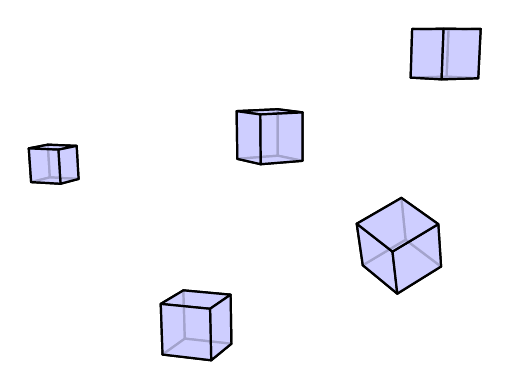
\begin{tikzpicture}[line join=round]
\filldraw[box](-3.055,1.164)--(-3.293,1.104)--(-3.323,1.532)--(-3.081,1.579)--cycle;
\filldraw[box](-3.055,1.164)--(-2.691,1.144)--(-2.715,1.564)--(-3.081,1.579)--cycle;
\filldraw[box](-3.055,1.164)--(-2.691,1.144)--(-2.92,1.083)--(-3.293,1.104)--cycle;
\filldraw[box](-3.081,1.579)--(-3.323,1.532)--(-2.947,1.516)--(-2.715,1.564)--cycle;
\filldraw[box](-2.691,1.144)--(-2.715,1.564)--(-2.947,1.516)--(-2.92,1.083)--cycle;
\filldraw[box](-3.323,1.532)--(-3.293,1.104)--(-2.92,1.083)--(-2.947,1.516)--cycle;
\filldraw[box](1.983,2.444)--(2.385,2.423)--(1.92,2.409)--(1.527,2.431)--cycle;
\filldraw[box](1.983,2.444)--(2.385,2.423)--(2.416,3.048)--(2.007,3.044)--cycle;
\filldraw[box](1.983,2.444)--(1.527,2.431)--(1.546,3.047)--(2.007,3.044)--cycle;
\filldraw[box](-.16,1.439)--(-.674,1.399)--(-.683,2.005)--(-.162,2.029)--cycle;
\filldraw[box](-.16,1.439)--(.152,1.374)--(.154,1.989)--(-.162,2.029)--cycle;
\filldraw[box](-.16,1.439)--(.152,1.374)--(-.377,1.331)--(-.674,1.399)--cycle;
\filldraw[box](2.007,3.044)--(1.546,3.047)--(1.945,3.051)--(2.416,3.048)--cycle;
\filldraw[box](-.162,2.029)--(-.683,2.005)--(-.382,1.963)--(.154,1.989)--cycle;
\filldraw[box](1.546,3.047)--(1.527,2.431)--(1.92,2.409)--(1.945,3.051)--cycle;
\filldraw[box](-.683,2.005)--(-.674,1.399)--(-.377,1.331)--(-.382,1.963)--cycle;
\filldraw[box](2.385,2.423)--(2.416,3.048)--(1.945,3.051)--(1.92,2.409)--cycle;
\filldraw[box](.152,1.374)--(.154,1.989)--(-.382,1.963)--(-.377,1.331)--cycle;
\filldraw[box](-1.341,-.884)--(-1.624,-1.086)--(-1.647,-.443)--(-1.359,-.271)--cycle;
\filldraw[box](-1.341,-.884)--(-.75,-.949)--(-.76,-.326)--(-1.359,-.271)--cycle;
\filldraw[box](-1.341,-.884)--(-.75,-.949)--(-1.006,-1.159)--(-1.624,-1.086)--cycle;
\filldraw[box](-1.359,-.271)--(-1.647,-.443)--(-1.021,-.505)--(-.76,-.326)--cycle;
\filldraw[box](-.75,-.949)--(-.76,-.326)--(-1.021,-.505)--(-1.006,-1.159)--cycle;
\filldraw[box](-1.647,-.443)--(-1.624,-1.086)--(-1.006,-1.159)--(-1.021,-.505)--cycle;
\filldraw[box](1.462,.372)--(1.913,.032)--(1.357,-.313)--(.919,.048)--cycle;
\filldraw[box](1.462,.372)--(1.913,.032)--(1.878,.57)--(1.409,.903)--cycle;
\filldraw[box](1.462,.372)--(.919,.048)--(.842,.575)--(1.409,.903)--cycle;
\filldraw[box](.842,.575)--(.919,.048)--(1.357,-.313)--(1.296,.221)--cycle;
\filldraw[box](1.913,.032)--(1.878,.57)--(1.296,.221)--(1.357,-.313)--cycle;
\filldraw[box](1.409,.903)--(.842,.575)--(1.296,.221)--(1.878,.57)--cycle;
\end{tikzpicture}% End sketch output

    \end{center}
}
\only<2-> {
    \begin{center}
    % Sketch output, version 0.3 (build 7d, Wed May 2 06:36:52 2012)
% Output language: PGF/TikZ,LaTeX
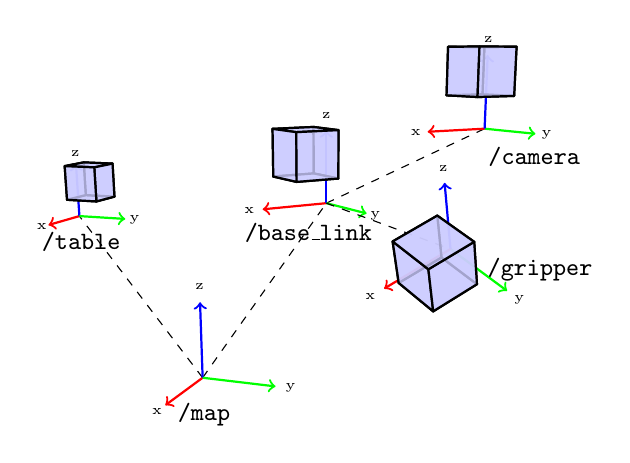
\begin{tikzpicture}[line join=round]
\draw[dashed](-1.571,-1.156)--(-3.136,.897);
\draw[axis,color=red,arrows=->](-3.136,.897)--(-3.529,.784);
\draw[axis,color=blue,arrows=->](-3.136,.897)--(-3.18,1.56);
\draw[axis,color=green,arrows=->](-3.136,.897)--(-2.553,.861);
\node at (-2.434,.854) {\tiny y};\node at (-3.189,1.695) {\tiny z};\node at (-3.613,.76) {\tiny x};\filldraw[box](-3.055,1.164)--(-2.691,1.144)--(-2.92,1.083)--(-3.293,1.104)--cycle;
\filldraw[box](-3.055,1.164)--(-2.691,1.144)--(-2.715,1.564)--(-3.081,1.579)--cycle;
\filldraw[box](-3.055,1.164)--(-3.293,1.104)--(-3.323,1.532)--(-3.081,1.579)--cycle;
\filldraw[box](-3.081,1.579)--(-3.323,1.532)--(-2.947,1.516)--(-2.715,1.564)--cycle;
\filldraw[box](-2.691,1.144)--(-2.715,1.564)--(-2.947,1.516)--(-2.92,1.083)--cycle;
\filldraw[box](-3.323,1.532)--(-3.293,1.104)--(-2.92,1.083)--(-2.947,1.516)--cycle;
\draw[axis,color=green,arrows=->](2.01,2.007)--(2.656,1.942);
\draw[dashed](0,1.061)--(2.01,2.007);
\draw[axis,color=red,arrows=->](2.01,2.007)--(1.287,1.968);
\draw[axis,color=blue,arrows=->](2.01,2.007)--(2.049,2.943);
\draw[dashed](-1.571,-1.156)--(0,1.061);
\draw[axis,color=red,arrows=->](0,1.061)--(-.809,.983);
\draw[axis,color=blue,arrows=->](0,1.061)--(0,1.984);
\draw[axis,color=green,arrows=->](0,1.061)--(.511,.931);
\draw[dashed](0,1.061)--(1.577,.478);
\filldraw[box](1.983,2.444)--(2.385,2.423)--(1.92,2.409)--(1.527,2.431)--cycle;
\filldraw[box](1.983,2.444)--(2.385,2.423)--(2.416,3.048)--(2.007,3.044)--cycle;
\filldraw[box](1.983,2.444)--(1.527,2.431)--(1.546,3.047)--(2.007,3.044)--cycle;
\filldraw[box](-.16,1.439)--(-.674,1.399)--(-.683,2.005)--(-.162,2.029)--cycle;
\filldraw[box](-.16,1.439)--(.152,1.374)--(.154,1.989)--(-.162,2.029)--cycle;
\filldraw[box](-.16,1.439)--(.152,1.374)--(-.377,1.331)--(-.674,1.399)--cycle;
\filldraw[box](2.007,3.044)--(1.546,3.047)--(1.945,3.051)--(2.416,3.048)--cycle;
\node at (2.796,1.928) {\tiny y};\node at (2.057,3.135) {\tiny z};\node at (1.135,1.96) {\tiny x};\filldraw[box](-.162,2.029)--(-.683,2.005)--(-.382,1.963)--(.154,1.989)--cycle;
\node at (.621,.903) {\tiny y};\node at (0,2.173) {\tiny z};\node at (-.979,.967) {\tiny x};\filldraw[box](1.546,3.047)--(1.527,2.431)--(1.92,2.409)--(1.945,3.051)--cycle;
\draw[axis,color=red,arrows=->](-1.571,-1.156)--(-2.045,-1.505);
\draw[axis,color=blue,arrows=->](-1.571,-1.156)--(-1.604,-.197);
\draw[axis,color=green,arrows=->](-1.571,-1.156)--(-.645,-1.266);
\filldraw[box](-.683,2.005)--(-.674,1.399)--(-.377,1.331)--(-.382,1.963)--cycle;
\filldraw[box](2.385,2.423)--(2.416,3.048)--(1.945,3.051)--(1.92,2.409)--cycle;
\filldraw[box](.152,1.374)--(.154,1.989)--(-.382,1.963)--(-.377,1.331)--cycle;
\node at (-.454,-1.289) {\tiny y};\node at (-1.611,0) {\tiny z};\node at (-2.15,-1.582) {\tiny x};\draw[axis,color=green,arrows=->](1.577,.478)--(2.296,-.053);
\draw[axis,color=blue,arrows=->](1.577,.478)--(1.502,1.32);
\draw[axis,color=red,arrows=->](1.577,.478)--(.734,-.024);
\node at (2.451,-.167) {\tiny y};\node at (1.485,1.502) {\tiny z};\node at (.56,-.128) {\tiny x};\filldraw[box](1.462,.372)--(1.913,.032)--(1.357,-.313)--(.919,.048)--cycle;
\filldraw[box](1.462,.372)--(1.913,.032)--(1.878,.57)--(1.409,.903)--cycle;
\filldraw[box](1.462,.372)--(.919,.048)--(.842,.575)--(1.409,.903)--cycle;
\filldraw[box](.842,.575)--(.919,.048)--(1.357,-.313)--(1.296,.221)--cycle;
\filldraw[box](1.913,.032)--(1.878,.57)--(1.296,.221)--(1.357,-.313)--cycle;
\filldraw[box](1.409,.903)--(.842,.575)--(1.296,.221)--(1.878,.57)--cycle;
\node at (-1.554,-1.62) {\small\tt /map};\node at (-3.114,.573) {\small\tt /table};\node at (-.229,.686) {\small\tt /base\_link};\node at (2.64,1.65) {\small\tt /camera};\node at (2.714,.211) {\small\tt /gripper};\end{tikzpicture}% End sketch output

    \end{center}
}

\only<2> {
    The \textbf{TF} library is responsible for maintaining the full
    transformation tree, and calculating the transformation between any two frames.
}
\only<3> {
    Attention: even though they look similar, frames and topics are unrelated.
}
\end{frame}

\begin{frame}{"Creating" frames}

Frames come to existence as soon as someone (a node) broadcast them.

\begin{center}
\resizebox{0.9\textwidth}{!}{%
\begin{tikzpicture}[
                    >=latex,
                    every edge/.style={->, draw, very thick},
                    service/.style={->, draw, very thick,dashed},
                    rosnode/.style={draw, font=\sf, node distance=0.5, rounded
                    corners, align=center, inner sep=5pt,fill=hriSec2Dark!50},
                    topic/.style={font=\tt, node distance=0.5, align=center, inner sep=5pt},
                    pic/.style={fill=none,draw=none}
                ]

    \node [rosnode] at (-2,1) (node1) {robot odometry};
    \node [rosnode] at (4,-2) (node2) {robot state publisher};
    \node [rosnode] at (-6,-4) (node3) {object tracker};

    \node [topic] at (-1,-1) (tf1) {/base\_link $\rightarrow$ /map};
    \node [topic] at (0,-5) (tf2) {/camera $\rightarrow$ /base\_link};
    \node [topic] at (-1,-4) (tf3) {/gripper $\rightarrow$ /base\_link};
    \node [topic] at (-4,-2) (tf4) {/table $\rightarrow$ /map};

    \path (node1) edge[bend left] node[label,right] {broadcasts} (tf1);
    \path (node2) edge[bend left] node[label,right] {broadcasts} (tf2);
    \path (node2) edge[bend right] (tf3);
    \path (node3) edge[bend left] node[label,left] {broadcasts} (tf4);

\end{tikzpicture}
}
\end{center}

\end{frame}

\begin{frame}[fragile]{How to write a TF broadcaster?}

    \begin{columns}
        \begin{column}{0.5\linewidth}
            \begin{center}C++
            \end{center}
\begin{minted}[frame=none,
        linenos=true,
        fontsize=\tiny,
        numbersep=0.4em,
        xleftmargin=0.5em]{cpp}

#include <ros/ros.h>
#include <tf/transform_broadcaster.h>


int main(int argc, char** argv){

  float x=0.f,y=0.f,theta=0.f;

  ros::init(argc, argv, "my_tf_broadcaster");
  tf::TransformBroadcaster br;
  ros::Rate rate(10); // 10 hz

  while (ros::ok()) {
    tf::Transform transform(
                    tf::Quaternion(0, 0, theta), 
                    tf::Vector3(x, y, 0.0));

    br.sendTransform(
         tf::StampedTransform(transform, 
                              ros::Time::now(), 
                              "my_robot", "map"));

    x++;
    rate.sleep();
  }
  return 0;
};
\end{minted}

            
        \end{column}
        \begin{column}{0.5\linewidth}
            \begin{center}Python
            \end{center}

\begin{minted}[frame=none,
               linenos=true,
               fontsize=\tiny,
               numbersep=0.4em,
               xleftmargin=0.5em]{python}

import rospy
import tf
from tf.transformations import quaternion_from_euler

if __name__ == '__main__':

   x = 0.; y = 0.; theta = 0.

   rospy.init_node('my_tf_broadcaster')
   br = tf.TransformBroadcaster()
   rate = rospy.Rate(10) # 10hz

   while not rospy.is_shutdown():

       br.sendTransform(
           (x, y, 0),
           quaternion_from_euler(0, 0, theta),
           rospy.Time.now(),
           "my_robot", "map")

       x += 1
       rate.sleep()

\end{minted}

            \vspace{2em}
        \end{column}
    \end{columns}

\end{frame}

%
%\begin{frame}[containsverbatim]{}
%
%\begin{shcode}
%> g++ tf.cpp -o tf -lroscpp -lrostime -lboost_system -ltf
%> ./tf
%\end{shcode}
%
%\end{frame}
%

\begin{frame}[containsverbatim]{}
\begin{shcode}
> rostopic echo tf
transforms: 
  - 
    header: 
      seq: 0
      stamp: 
        secs: 1449488936
        nsecs: 480597909
      frame_id: map
    child_frame_id: my_robot
    transform: 
      translation: 
        x: 239.0
        y: 0.0
        z: 0.0
      rotation: 
        x: 0.0
        y: 0.0
        z: 0.0
        w: 1.0
---

\end{shcode}

\end{frame}

\begin{frame}{To summarize: key concepts}
    \begin{itemize}
        \item Node
        \item Master
        \item Messages
        \item Topics
        \item Services
        \item Actions
        \item Transformations/frames
    \end{itemize}

    \pause

    Some additional concepts that we will discuss later on:
    \begin{itemize}
        \item Package
        \item Launch file
    \end{itemize}
\end{frame}

%%%%%%%%%%%%%%%%%%%%%%%%%%%%%%%%%%%%%%%%%%%%%%%%%%%%%%%%%%%%%%%%%%%%%%%%%%%%%%%%%%%
%%%%%%%%%%%%%%%%%%%%%%%%%%%%%%%%%%%%%%%%%%%%%%%%%%%%%%%%%%%%%%%%%%%%%%%%%%%%%%%%%%%
%%%%%%%%%%%%%%%%%%%%%%%%%%%%%%%%%%%%%%%%%%%%%%%%%%%%%%%%%%%%%%%%%%%%%%%%%%%%%%%%%%%

\section[Robot arm]{Example: a robotic arm with ROS}

\imageframe[caption={That's our hardware...}, color=black]{servo-arm2}
\imageframe[caption={That's what we want...}, color=black]{servo-rviz}

\begin{frame}{Nodes}

\begin{center}
\begin{tikzpicture}[
                    >=latex,
                    every edge/.style={->, draw, very thick},
                    service/.style={->, draw, very thick,dashed},
                    rosnode/.style={draw, font=\sf, node distance=0.5, rounded corners, align=center, inner sep=5pt,fill=hriSec2Dark!50},
                    servo/.style={draw, font=\sf, node distance=0.5, align=center, inner sep=5pt,fill=hriSec3Comp!50},
                    topic/.style={font=\tt, node distance=0.5, align=center, inner sep=5pt},
                    pic/.style={fill=none,draw=none}
                ]

    \path[use as bounding box] (-6,1) rectangle (6,-5);

    \only<1-2>{
    \node [rosnode] at (0,0) (node1) {servo ctrl 1};
    \node [servo,above=0.3 of node1] (node1s) {servo};
    \path[<->,thick] (node1) edge (node1s);
    \node [rosnode] at (4,-2) (node2) {servo ctrl 2};
    \node [servo,above=0.3 of node2] (node2s) {servo};
    \path[<->,thick] (node2) edge (node2s);
    }
    \only<3>{
        \node [rosnode] at (0,0) (node1) {servos ctrl -- \textbf{Arduino}};
        \node [servo,above=0.3 of node1] (node1s) {servo};
        \path[<->,thick] (node1) edge (node1s);
        \node [servo,right=0.3 of node1s] (node2s) {servo};
        \path[<->,thick] (node1) edge (node2s);
    }

    \node [rosnode] at (-5,-4) (node3) {viz 3D\only<3>{ -- \texttt{rviz}}};
    \node [rosnode] at (0,-4) (node4) {GUI\only<3>{ -- \texttt{joint\_state\_publisher}}};

    \uncover<2-> {
        \node [topic] at (0,-2) (topic1) {/joint\_states};
        \path (node4) edge[bend left] (topic1);
        \path (topic1) edge[bend right] (node1);
        \path<2> (topic1) edge[bend right] (node2);
        \path (topic1) edge[bend right] (node3);
    }

    \only<1>{
        \node [rosnode,fill=hriSec3!50] at (-5,0) (roscore) {roscore};
        \path[dashed] (node1) edge[<->,very thin, bend right] node[label,above] {} (roscore);
        \path[dashed] (node2) edge[<->,very thin, bend right] node[label,above] {} (roscore);
        \path[dashed] (node3) edge[<->,very thin, bend left] node[label,above right] {} (roscore);
        \path[dashed] (node4) edge[<->,very thin, bend left] node[label,above right] {} (roscore);
    }

\end{tikzpicture}
\end{center}

\end{frame}


\begin{frame}[fragile]{ROS with the Arduino}

    \sh{rosserial} is a ROS \emph{bridge} that transparently transport ROS messages
    over a serial connection.

    \sh{rosserial_arduino} is a \sh{rosserial} \emph{client} for the Arduino.
    You can install it easily:\\
    \sh{apt install ros-kinetic-rosserial ros-kinetic-rosserial-arduino}

    To make it transparently available in the Arduino IDE, you need to also
    install it as an Arduino library:

    \begin{shcode}
> cd $HOME/sketchbook/libraries
> rosrun rosserial_arduino make_libraries.py .
    \end{shcode}
\end{frame}

\imageframe{arduino-ide-ros}

\begin{frame}[fragile]{Arduino code to control a servo with ROS}
\begin{columns}
    \begin{column}{0.5\linewidth}
        
\begin{minted}[frame=none,
        linenos=true,
        fontsize=\tiny,
        numbersep=0.4em,
        xleftmargin=0.5em]{cpp}
#include <ros.h>
#include <std_msgs/UInt16.h>
#include <Servo.h> 

using namespace ros;

NodeHandle  nh;
Servo servo;

void cb( const std_msgs::UInt16& msg){
  servo.write(msg.data); // 0-180
}

Subscriber<std_msgs::UInt16> sub("servo", cb);

void setup(){
  nh.initNode();
  nh.subscribe(sub);

  servo.attach(9); //attach it to pin 9
}

void loop(){
  nh.spinOnce();
  delay(1);
}
\end{minted}
    \end{column}
    \begin{column}{0.5\linewidth}

        \small Python $\approx$equivalent:

\begin{minted}[frame=none,
               linenos=true,
               fontsize=\tiny,
               numbersep=0.4em,
               xleftmargin=0.5em]{python}
import rospy
from std_msgs.msg import UInt16

def cb(msg):
    # servo.write(msg.data)
    print(msg.data)

rospy.init_node('listener')
rospy.Subscriber("servo", UInt16, cb)
# servo.attach(9)
rospy.spin()
\end{minted}
    \end{column}
\end{columns}
\end{frame}

\begin{frame}[fragile]{Running the code}
    To use the code, from your 'master' ROS computer:

\begin{shcode}
> roscore
> rosrun rosserial_python serial_node.py /dev/ttyACM0
> rostopic pub --once servo std_msgs/UInt16 110
\end{shcode}
\end{frame}


\begin{frame}{URDF}

        \textbf{URDF} (\emph{Unified Robot Description Format}) is an XML-based language
        to describe a robot.

        \begin{columns}
            \begin{column}{0.5\linewidth}
        \begin{center}
            \includegraphics[width=0.8\linewidth]{link}
        \end{center}
                
            \end{column}
            \begin{column}{0.5\linewidth}
        \begin{itemize}
                \small
            \item Primitives (cylinders, cubes, spheres) to describe the
                geometry
            \item For complex geometries, any STL or Collada meshes can be used
            \item Only \emph{tree structures} can be represented: no parallel robots
            \item Only \emph{rigid links} can be represented: no soft robots
        \end{itemize}
            \end{column}
        \end{columns}
\end{frame}

\begin{frame}[fragile]{URDF: Describing the kinematics of our robot}

    \begin{columns}
        \begin{column}{0.5\linewidth}
    \begin{overprint}
        \onslide<1>

    \begin{minted}[frame=none,
               fontsize=\tiny,
               numbersep=0.4em,
               xleftmargin=0.5em]{xml}
<?xml version="1.0"?>
<robot name="roco_arm">
  <link name="base_link">
    <visual>
      <geometry>
        <cylinder length="0.06" radius="0.1"/>
      </geometry>
    </visual>
  </link>


















</robot>
\end{minted}

        \onslide<2>
    \begin{minted}[frame=none,
               fontsize=\tiny,
               numbersep=0.4em,
               xleftmargin=0.5em]{xml}
<?xml version="1.0"?>
<robot name="roco_arm">
  <link name="base_link">
    <visual>
      <geometry>
        <cylinder length="0.06" radius="0.1"/>
      </geometry>
    </visual>
  </link>

  <link name="first_segment">
    <visual>
      <geometry>
        <box size="0.6 0.05 0.1"/>
      </geometry>
      <origin rpy="0 0 0" xyz="-0.3 0 0" />
    </visual>
  </link>









</robot>
\end{minted}

        \onslide<3>
    \begin{minted}[frame=none,
               fontsize=\tiny,
               numbersep=0.4em,
               xleftmargin=0.5em]{xml}
<?xml version="1.0"?>
<robot name="roco_arm">
  <link name="base_link">
    <visual>
      <geometry>
        <cylinder length="0.06" radius="0.1"/>
      </geometry>
    </visual>
  </link>

  <link name="first_segment">
    <visual>
      <geometry>
        <box size="0.6 0.05 0.1"/>
      </geometry>
      <origin rpy="0 0 0" xyz="-0.3 0 0" />
    </visual>
  </link>

  <joint name="base_to_first" type="revolute">
    <axis xyz="0 1 0" />
    <limit effort="1000" lower="0"
                    upper="3.14" velocity="0.5" />
    <parent link="base_link"/>
    <child link="first_segment"/>
    <origin xyz="0 0 0.03" />
  </joint>
</robot>
\end{minted}

    \end{overprint}
        \end{column}
        \begin{column}{0.5\linewidth}
            \begin{center}
                \includegraphics[width=0.8\linewidth]{servo-arm2-narrow}
            \end{center}
        \end{column}
    \end{columns}
\end{frame}


\begin{frame}[fragile]{Display the model}

    To display and interact with the URDF model:

    \begin{minted}[fontsize=\footnotesize]{sh}
> rosparam set robot_description -t code/robot-arm.urdf
> rosrun robot_state_publisher robot_state_publisher
> rosrun joint_state_publisher joint_state_publisher _use_gui:=true
> rosrun rviz rviz
\end{minted}
\end{frame}

\imageframe{urdf-rviz}

\begin{frame}[plain]

\begin{center}
    \resizebox{0.7\linewidth}{!}{%
\begin{tikzpicture}[
                    >=latex,
                    every edge/.style={->, draw, very thick},
                    service/.style={->, draw, very thick,dashed},
                    rosnode/.style={draw, font=\sf, node distance=0.5, rounded corners, align=center, inner sep=5pt,fill=hriSec2Dark!50},
                    servo/.style={draw, font=\sf, node distance=0.5, align=center, inner sep=5pt,fill=hriSec3Comp!50},
                    topic/.style={font=\tt, node distance=0.5, align=center, inner sep=5pt},
                    pic/.style={fill=none,draw=none}
                ]

    \path[use as bounding box] (-6,1) rectangle (6,-5);

        \node [rosnode] at (0,0) (node1) {servos ctrl -- \textbf{Arduino}};
        \node [servo,above=0.3 of node1] (node1s) {servo};
        \path[<->,thick] (node1) edge (node1s);
        \node [servo,right=0.3 of node1s] (node2s) {servo};
        \path[<->,thick] (node1) edge (node2s);

    \node [rosnode] at (-5,-4) (node3) {viz 3D -- \texttt{rviz}};
    \node [rosnode] at (0,-4) (node4) {GUI -- \texttt{joint\_state\_publisher}};

        \node [topic] at (0,-2) (topic1) {/joint\_states};
        \path (node4) edge[bend left] (topic1);
        \path (topic1) edge[bend right] (node1);

    \only<1-2>{
        \path (topic1) edge[bend right] (node3);
    }

    \only<3>{
        \node [rosnode,above=2.5 of node3] (node5) {\texttt{robot\_state\_publisher}};
        \node [topic, above=1 of node3] (topic2) {/tf};
        \path (topic1) edge[bend right] (node5);
        \path (node5) edge (topic2);
        \path (topic2) edge (node3);
    }

\end{tikzpicture}
}

        Why do we need \texttt{robot\_state\_publisher}?
    \end{center}

    \only<2>

    \texttt{rviz} needs the {transformations} between each geometry.
    Going from a \textbf{joint state} (\ie the angles for each joint) to
    transformations (\ie \textbf{frames}) requires \textbf{forward kinematics}.

    \only<3>
        \texttt{robot\_state\_publisher} \emph{subscribes} to the joint state
        topic \texttt{/joint\_states} and \emph{broadcasts} the corresponding TF
        frames.

\end{frame}

\begin{frame}[fragile]{Joint state}
\begin{shcode}
> rosmsg show sensor_msgs/JointState 
std_msgs/Header header
  uint32 seq
  time stamp
  string frame_id
string[] name
float64[] position
float64[] velocity
float64[] effort
\end{shcode}

\source{http://docs.ros.org/api/sensor_msgs/html/msg/JointState.html}{sensor\_msgs::JointState definition}
\end{frame}


\begin{frame}[fragile]{Reading the joint state on an Arduino}
\begin{columns}
    \begin{column}{0.5\linewidth}

\small Original: reading an integer
\begin{minted}[frame=none,
        linenos=true,
        fontsize=\tiny,
        numbersep=0.4em,
        xleftmargin=0.5em]{cpp}
#include <ros.h>
#include <std_msgs/UInt16.h>
#include <Servo.h> 

using namespace ros;

NodeHandle  nh;
Servo servo;

void cb( const std_msgs::UInt16& msg){
  servo.write(msg.data); // 0-180
}


Subscriber<std_msgs::UInt16> 
                        sub("servo", cb);

void setup(){
  nh.initNode();
  nh.subscribe(sub);

  servo.attach(9); //attach it to pin 9
}

void loop(){
  nh.spinOnce();
  delay(1);
}
\end{minted}
    \end{column}
    \begin{column}{0.5\linewidth}

\small Updated: reading the joint state

\begin{minted}[frame=none,
        linenos=true,
        fontsize=\tiny,
        numbersep=0.4em,
        xleftmargin=0.5em]{cpp}
#include <Servo.h> 
#include <ros.h>
#include <sensor_msgs/JointState.h>

using namespace ros;

NodeHandle  nh;
Servo servo;

void cb( const sensor_msgs::JointState& msg){
  int angle = (int) (msg.position[0] * 180/3.14);
  servo.write(angle); // 0-180
}

Subscriber<sensor_msgs::JointState>
                        sub("joint_states", cb);

void setup(){
  nh.initNode();
  nh.subscribe(sub);
  
  servo.attach(9); //attach it to pin 9
}

void loop(){
  nh.spinOnce();
  delay(1);
}
\end{minted}



    \end{column}
\end{columns}
\end{frame}



%%%%%%%%%%%%%%%%%%%%%%%%%%%%%%%%%%%%%%%%%%%%%%%%%%%%%%%%%%%%%%%%%%%%%%%%%%%%%%%%%%%%
%%%%%%%%%%%%%%%%%%%%%%%%%%%%%%%%%%%%%%%%%%%%%%%%%%%%%%%%%%%%%%%%%%%%%%%%%%%%%%%%%%%%
%%%%%%%%%%%%%%%%%%%%%%%%%%%%%%%%%%%%%%%%%%%%%%%%%%%%%%%%%%%%%%%%%%%%%%%%%%%%%%%%%%%%
\section[Code]{Code management}

\begin{frame}[fragile]{Packages}

The source code of ROS nodes is usually organised into a \emph{package}.

\begin{shcode}
> cd my_package
> ls
CMakeLists.txt  # describes the build process
cfg/  # node specific configurations
include/  # C/C++ public headers
launch/  # ROS launch files
msgs/  # custom datatypes (messages)
scripts/  # executable scripts, typically Python ROS nodes
package.xml  # package manifest
src/  # source code of your node
> rosrun my_package my_node
\end{shcode}

\only<1>{
One package often contains more than one node.

Besides the source code, packages may contain as well specific messages,
configuration files, launch files, etc.
}

\only<2>{
Packages must contain a \emph{manifest}, \texttt{package.xml}. It contains the
package name, version, authors, as well as the dependencies.
}

\only<3>{

A new package template can be created easily:

\texttt{> catkin\_create\_pkg my\_package <ROS dependencies>}

}
\end{frame}

\begin{frame}[fragile]{Creating a ROS package, step by step}

Let's turn the initial 'image processing' example into a proper ROS package.

\begin{shcode}
> cd $HOME
> mkdir src && cd src
> catkin_create_pkg imgproc rospy
\end{shcode}
\pause
\begin{shcode}
> ls imgproc
CMakeLists.txt  package.xml  src
\end{shcode}

\end{frame}

\begin{frame}[fragile]{First, add some code}

\begin{shcode}
> cd imgproc  # we now are in $HOME/src/imgproc
> mkdir -p src/imgproc
> cd src/imgproc # we now are in $HOME/src/imgproc/src/imgproc
> touch __init__.py # required to create a Python module
> gedit processing.py
\end{shcode}
\pause

Initially, we simply create a stub of our Python module for image processing:

\begin{pythoncode}
def process(image):
    print('Image to be processed: ' + image)
\end{pythoncode}

\end{frame}

\begin{frame}[fragile]{First, add some initial code}

We create as well an executable (our future ROS node) in \texttt{scripts/}:

\begin{shcode}
> cd ../..  # we now are back to $HOME/src/imgproc
> mkdir -p scripts && cd scripts
> gedit process_node
\end{shcode}
\pause

\begin{pythoncode}
#! /usr/bin/env python

import imgproc.processing

imgproc.processing.process("my_image")
\end{pythoncode}

\pause

Finally, we make our script executable:
\begin{shcode}
> chmod +x process_node
\end{shcode}
\end{frame}

\begin{frame}[fragile]{Configure the Python 'build'}

Because our node is written in Python, our \texttt{CMakeLists.txt} is simple:

\begin{cmakecode}
cmake_minimum_required(VERSION 2.8.3)
project(imgproc)

find_package(catkin REQUIRED COMPONENTS
  rospy
)

catkin_python_setup()
catkin_package()

install(PROGRAMS
   scripts/process_node
   DESTINATION ${CATKIN_PACKAGE_BIN_DESTINATION}
)

\end{cmakecode}
\end{frame}

\begin{frame}[fragile]{Configure the Python 'build'}

However, we need a \texttt{setup.py} (standard Python
    \texttt{distutils}-based packaging):

\begin{pythoncode}
from distutils.core import setup
from catkin_pkg.python_setup import generate_distutils_setup

# fetch values from package.xml
setup_args = generate_distutils_setup(
                    packages=['imgproc'],
                    package_dir={'': 'src'},
                )

setup(**setup_args)
\end{pythoncode}

\end{frame}

\begin{frame}[fragile]{Install the node}

    We can now install our node:

\begin{shcode}
> cd $HOME/src/imgproc  # back to the root of our ROS pkg
> mkdir -p build && cd build
> cmake -DCMAKE_INSTALL_PREFIX=<install prefix> ..
> make install
\end{shcode}

\pause

Assuming ROS is correctly installed, we can run our node:

\begin{shcode}
> export ROS_PACKAGE_PATH=<prefix>/share:$ROS_PACKAGE_PATH
> rosrun imgproc process_node
Dataset: my_image
\end{shcode}

Add the \sh{export ROS_PACKAGE_PATH...} line to the end of your
\sh{~/.bashrc} file, so that you do not have to type it everytime.

\end{frame}

\begin{frame}[fragile]{Image processing}
Let's update the node \texttt{reco} and the library (Python \emph{module})
    \texttt{processing.py} to perform simple image processing:

\texttt{processing.py}:
\begin{pythoncode}
import cv2

def process(image):
    rows, cols, channels = image.shape
    cv2.circle(image, (cols/2, rows/2), 50, (0,0,255), -1)
\end{pythoncode}
\end{frame}

\begin{frame}[fragile]{Image processing}
\texttt{process\_node}:
\begin{pythoncode}
#! /usr/bin/env python

import sys, rospy
from sensor_msgs.msg import Image
from cv_bridge import CvBridge

import imgproc.processing

def on_image(image):
    cv_image = bridge.imgmsg_to_cv2(image, "bgr8")
    imgproc.processing.process(cv_image)
    image_pub.publish(bridge.cv2_to_imgmsg(cv_image, "bgr8"))

if __name__ == '__main__':
    rospy.init_node('image_processor')
    bridge = CvBridge()
    image_sub = rospy.Subscriber("image",Image, on_image)
    image_pub = rospy.Publisher("processed_image",Image, queue_size=1)

    while not rospy.is_shutdown():
        rospy.spin()
\end{pythoncode}

\end{frame}

\begin{frame}[fragile]{To use the node}


\begin{shcode}
> rosrun usb_cam usb_cam_node
\end{shcode}


\begin{shcode}
> rosrun imgproc process_node image:=/usb_cam/image_raw
\end{shcode}


\begin{shcode}
> rqt_image_view image:=/processed_image
\end{shcode}

\end{frame}


\begin{frame}[plain]
    \begin{center}
        \Large
    Let's try it!
    \end{center}
\end{frame}

\begin{frame}[fragile]{Launch files}
\only<1>{
\emph{Launch files} allow to group together nodes and their configuration.
}

\begin{minted}[fontsize=\footnotesize]{xml}
<launch>
  <arg name="model" />
  <arg name="gui" default="true" />

  <param name="robot_description" textfile="$(arg model)" />
  <param name="use_gui" value="$(arg gui)"/>

  <node name="joint_state_publisher" pkg="joint_state_publisher" 
                                type="joint_state_publisher" />
  <node name="robot_state_publisher" pkg="robot_state_publisher" 
                                type="state_publisher" />
  <node name="rviz" pkg="rviz" type="rviz" required="true" />

</launch>
\end{minted}


\only<2>{
    To use the launch file, call \texttt{roslaunch} instead of \texttt{rosrun}:

    \texttt{> roslaunch my\_package interactive\_arm.launch}
}
\only<3>{
    Arguments (\texttt{<arg>}) can be provided from the command-line:

    \texttt{> roslaunch my\_package interactive\_arm.launch model:=my\_arm.urdf}
}
\only<4>{
    Parameters (\texttt{<param>}) are loaded to the ROS \emph{parameter server}
    and shared with all the ROS nodes.
}
\only<5>{
    Some nodes may be marked as \texttt{required}: if they die (closed or crashed),
    all the other nodes in the launch file are killed as well.
}
\only<6>{
    Many more possibilities, see \href{http://wiki.ros.org/roslaunch/XML}{roslaunch
    documentation}.
}
\end{frame}

\section{Tools}

\imageframe[color=black]{rviz}
\imageframe[color=black]{rviz-plugins}
\imageframe[color=black]{urdf-rviz}
\imageframe[color=black]{rviz-sandtray}
\imageframe[color=black]{rviz-pointcloud}
\imageframe[color=black]{rviz-faces}


\begin{frame}{Other tools}
    \begin{table}[]
        \begin{tabularx}{\linewidth}{l>{\raggedright}X}
            \toprule
            \texttt{rosnode}, \texttt{rostopic},... & Print out/publish/call messages, services, nodes \tabularnewline
            \texttt{rosconsole} & Centralized logging \tabularnewline
            \texttt{rosbag} & Record and replay messages \tabularnewline
            \texttt{rqt\_reconfigure} & Live configuration of nodes \tabularnewline
            \texttt{rqt\_diagnostics} & Standardized diagnostics \tabularnewline
            \texttt{rosgraph} & plots the node network \tabularnewline
            \bottomrule
        \end{tabularx}
    \end{table}
\end{frame}

\begin{frame}[fragile]{}
\begin{shcode}
> rosnode list 
/camera_base_link
/camera_base_link1
/camera_base_link2
/camera_base_link3
/ros_attention_tracker
/rosout
/camera/camera_nodelet_manager
/camera/debayer
/camera/depth_metric
/camera/depth_metric_rect
/camera/depth_points
/camera/depth_rectify_depth
/camera/depth_registered_hw_metric_rect
/camera/depth_registered_metric
/camera/depth_registered_rectify_depth
/camera/depth_registered_sw_metric_rect
/camera/disparity_depth
/camera/disparity_registered_hw
/camera/disparity_registered_sw
/camera/driver
/camera/points_xyzrgb_hw_registered
/camera/points_xyzrgb_sw_registered
/camera/rectify_color
/camera/rectify_ir
/camera/rectify_mono
/camera/register_depth_rgb
\end{shcode}

\end{frame}

\begin{frame}[fragile]{}
\begin{shcode}
> rostopic list
/camera_info
/image
/nb_detected_faces
/rosout
/rosout_agg
/tf
/camera/depth/image_rect_raw
/camera/depth/image_rect_raw/compressed
/camera/depth/image_rect_raw/compressed/parameter_descriptions
/camera/depth/image_rect_raw/compressed/parameter_updates
/camera/depth/image_rect_raw/compressedDepth
/camera/depth/image_rect_raw/compressedDepth/parameter_descriptions
/camera/depth/image_rect_raw/compressedDepth/parameter_updates
/camera/depth/image_rect_raw/theora
/camera/depth/image_rect_raw/theora/parameter_descriptions
/camera/depth/image_rect_raw/theora/parameter_updates
/camera/depth_rectify_depth/parameter_descriptions
/camera/depth_rectify_depth/parameter_updates
\end{shcode}

\end{frame}

\begin{frame}[fragile]{}
\begin{shcode}
> rostopic echo tf
transforms: 
  - 
    header: 
      seq: 0
      stamp: 
        secs: 1449222890
        nsecs: 396561780
      frame_id: /camera_link
    child_frame_id: /camera_rgb_frame
    transform: 
      translation: 
        x: 0.0
        y: -0.045
        z: 0.0
      rotation: 
        x: 0.0
        y: 0.0
        z: 0.0
        w: 1.0
---
transforms: 
  - 
    header: 
      seq: 0
      stamp: 
        secs: 1449222890

\end{shcode}

\end{frame}

\imageframe[color=black]{console}
\imageframe[color=black]{bag}
\imageframe[color=black]{dynamic_reconfigure}

\section[Doc]{ROS documentation}

\begin{frame}{ROS documentation}

Plenty!

Some examples:

\begin{itemize}
    \item Tutorial: \href{http://wiki.ros.org/ROS/Tutorials}{wiki.ros.org/ROS/Tutorials}
    \item Supported robots: \href{http://robots.ros.org/}{robots.ros.org}
    \item Message definition example:
        \href{http://docs.ros.org/api/sensor_msgs/html/msg/LaserScan.html}{sensor\_msgs/LaserScan}
    \item Node documentation example:
        \href{http://wiki.ros.org/face_detector}{wiki.ros.org/face\_detector}
\end{itemize}
\end{frame}

\section[So?]{So, what is ROS?}

\begin{frame}{ROS is...}
    \begin{itemize}
        \item<+-> A fairly simple peer-to-peer message passing system designed with robotics in
            mind
        \item<+-> An API to this system (in several languages -- C++ and Python are
            1st tier)
        \item<+-> A set of standard message types that facilitate interoperability between modules
        \item<+-> A set of conventions to write and package robotic softwares
        \item<+-> Deep integration of a few key open-source libraries (OpenCV, PCL, tf)
        \item<+-> A set of tools to run and monitor the nodes
    \end{itemize}
\end{frame}


\begin{frame}{}
    \begin{center}
        \Large
        That's all, folks!\\[2em]
    \end{center}
        \vspace{10em}

        Slides:\\ 
        \href{https://github.com/severin-lemaignan/ros-presentation}{\small github.com/severin-lemaignan/ros-presentation}

\end{frame}



\end{document}
